\setcounter{chapter}{1}
\chapter[Inversion and forward estimation with process-based hazard models: an investigation into cost functions, uncertainty-based weights and model-data fusion]{Inversion and forward estimation with process-based hazard models: an investigation into cost functions, uncertainty-based weights and model-data fusion}\label{chap-tephra}

\begin{small}
This chapter is a journal article under review. Appendix \ref{app-tephra} pertains to the Supplementary Material submitted with the paper.
\\
\\
\noindent
\textbf{Rabonza M.L.}, Nguyen M., Biasse S., Jenkins S., Taisne B., Lallemant D., (2023) Inversion and forward estimation with process-based models: an investigation into cost functions, uncertainty-based weights and model-data fusion. \textit{Environmental Modelling & Software}, Under review.

%----------------
% \section*{Highlights}
% %--- RESEARCH HIGHLIGHTS
% %----------------
% \begin{itemize}
% \item I propose a two-step approach to evaluate the choice of cost function in inversion.

% \item I demonstrate a calibration approach that weighs observations in the cost function based on data uncertainty.

% \item I present an improvement to spatial estimation that combines the forward model output and data.

% \item I demonstrate the methods using a tephra fallout model.
% \end{itemize}

%%% Start of highlights
\clearpage
\vspace*{\fill}
\begingroup
\centering

\textbf{\Large{Chapter highlights}}

\hrulefill 

\begin{itemize}
\item \textsl{I propose a two-step approach to evaluate the choice of cost function in inversion.}

\item \textsl{I demonstrate a calibration approach that weighs observations in the cost function based on data uncertainty.}

\item \textsl{I present an improvement to spatial estimation that combines the forward model output and data.}

\item \textsl{I demonstrate the methods using a tephra fallout model.}
\end{itemize}


\endgroup
\vspace*{\fill}
%%% End of Highlights



% %----------------
% \vspace{2cm}
% \noindent
% \textbf{Keywords:} Tephra; Inversion; Model calibration; Kriging; Kelud volcano

\end{small}
\clearpage
%%%%%%%%%%%%%%%%%
\section{Abstract}

Process-based models for inversion and forward estimation have supported our understanding of earth, environment, and hazards processes. These methods are often applied on spatial data without accounting for their spatial nature and uncertainty. Using an example of reconstructing past volcanic eruption characteristics and associated tephra fallout from different sets of field observation, we demonstrate the importance of making the best use of data-related uncertainty and spatial information in inversion and forward estimation. We present strategies for: (1) the selection of appropriate cost functions accounting for their behaviour and implied distribution of residuals, (2) the treatment of differential uncertainty when combining multiple data, and (3) the leveraging of both model and data when estimating the spatial distribution of output. Results show that a data-informed choice of cost function and accounting for uncertainty and spatial characteristics of data leads to consistent improvements in model predictive performance for both inversion and forward models. %150


%%%%%%%%%%%%%%%%%%%%%%%%%%%%%%%%%%%%%%%%%%%%%%%%%%


%----------------
\section{Introduction}\label{section-intro}
% State the objectives of the work and provide an adequate background, avoiding a detailed literature survey or a summary of the results.
%----------------

Process-based models are important tools used to represent physical phenomena and processes in natural hazards analysis. In the \textit{inversion or calibration setting}, they are used to estimate parameters that cannot be directly measured, through calibration to the observed response of the hazard system. Examples include estimating floodplain characteristics based on observations of past floods, estimating earthquake rupture characteristics based on recordings from seismic stations, or estimating volcanic eruption source parameters based on measurements of the deposited tephra (ejected particles of all sizes) across the impacted region \citep{li2022comparative, georgoudas2007cellular, connor2006inversion}. In the \textit{forward estimation setting}, process-based models are used to estimate the \textit{response} of the hazard system based on calibrated or assumed parameters. Examples include flood simulation using a calibrated inundation model, estimating ground-motion intensity for a given earthquake magnitude and location, or estimating tephra accumulation given eruption and wind parameters \citep{uhlenbrook2004hydrological, worden2010revised, wang2022ground, hurst1999performance, folch2009fall3d}. Such applications of inversion and forward estimation frameworks merge the imperfect knowledge derived from data with that of process-based models in a way that utilises the reinforcing characteristics of both models and data.

As attention turns to such learning-from-data problems, recent advancements in optimisation and uncertainty quantification underline the issue of treating inversion-forward estimation problems with a black-box perspective that ignores the characteristics of both models and data \citep{hollos2022conditional, cabaneros2022methods, biegler2011large, ISAAC2015348, oden2010computer}. Despite technological improvements in the collection of observed data (e.g. remote sensing) and the increasing complexity of newly-developed process-based models, inversion-forward estimation frameworks often ignore particular characteristics in the data that they rely on (e.g. distribution, uncertainty, and spatial properties; \cite{willcox2021imperative}). Thus, there is a need to be strategic about how the inversion-forward estimation framework uses limited and uncertain data.

In this paper, we study this issue using the example of reconstructing past volcanic eruption characteristics and associated tephra fallout from observations across the impacted area. The application follows a typical inversion-forward estimation workflow shown in Figure \ref{fig:schem-typ}. The inversion and forward estimation workflows can be conducted sequentially, as visualized in Figure \ref{fig:schem-typ}, or separately. In the inversion/calibration setting, tephra fallout models are used to estimate eruption source parameters (ESPs, e.g. tephra mass, total grain size distribution, plume height, and plume profile) and empirical parameters (e.g. fall–time threshold, diffusion coefficient) from observations of tephra characteristics such as deposit thickness and grain size, typically collected through field surveys in the impacted area. As in any inversion process, an automated search routine finds the parameters of a model in such a way that the modelled response best approximates the observed data. The search routine optimises a \textit{cost function} (also known as loss function or objective function), which calculates the agreement between the model estimates of tephra deposits and the observations. This process can estimate eruption parameters for past events, which is an important input for estimating the potential size and intensity of future eruptions, and their associated consequences \citep{newhall1982volcanic, carey1986quantitative, pieri1986eruption, armienti1988numerical, scarpati1993neapolitan, mastin2009multidisciplinary, stohl2011determination, pouget2013estimation, madankan2014computation, bear2020automated}. In the forward estimation setting, tephra fallout models can map the distribution of tephra accumulation. The map can serve multiple purposes, including estimating eruption impacts on communities \citep{le2012, wardman2012, magill2013, biass2017}, assessing the vulnerability of buildings to tephra loading \citep{williams2020, HAYES2019142, spence2005}, or quantifying risk to agriculture \citep{gomez2006, ayris2012, thompson2017}. 

%%%%%
\begin{figure*}[htbp]
\centering
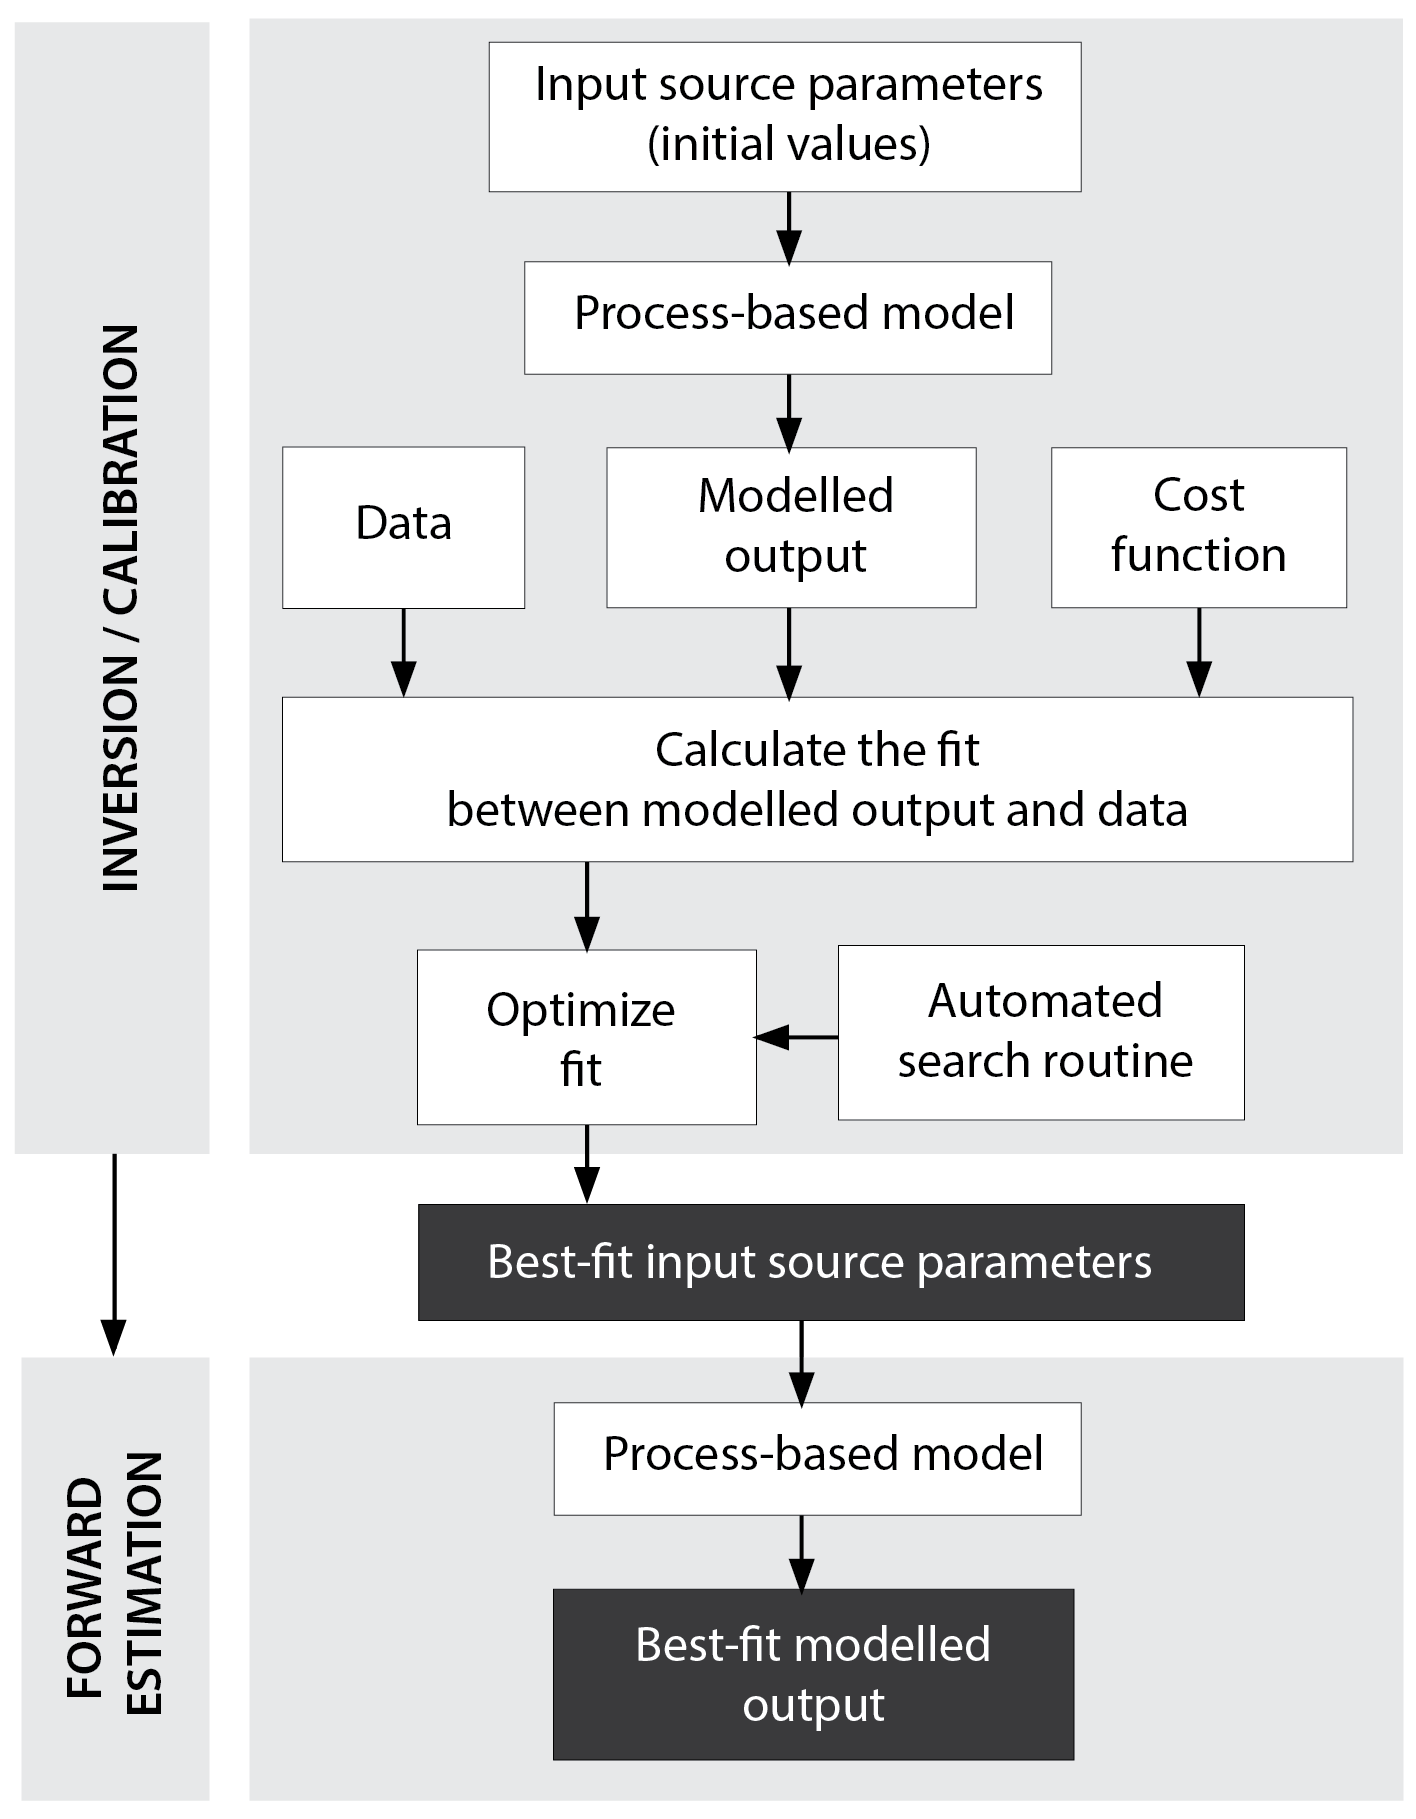
\includegraphics[width=.8\linewidth]{Figures/fig1_schematic.png}
\caption{Schematic of a typical inversion-forward estimation workflow using a process-based model. The purpose of the inversion is to estimate the best-fit input source parameters (e.g. erupted mass, plume height), while the purpose of forward estimation is to obtain best-fit modelled outputs (e.g. a map of the tephra thickness). The inversion and estimation workflows can be conducted sequentially, as visualised here, or conducted separately/independently. The outputs of the inversion and estimation are shown as black boxes.}
\label{fig:schem-typ}
\end{figure*}

Given the importance and broad applicability of process-based models, this study focuses not on the models themselves, but on how they are calibrated with limited and uncertain data and how they can best utilise such data in both inversion/calibration and forward estimation settings. We explore these through the study of tephra fallout from the 2014 eruption of Kelud volcano and the use of the \textit{Tephra2} model of \cite{bonadonna2005probabilistic} as the process-based model. \cite{connor2006inversion}'s algorithm is followed for the inversion workflow. The study does not make any particular claim or conclusions about the characteristics of the Kelud eruption or the accuracy of the \textit{Tephra2}, both of which have been extensively studied by others \citep{MAENO201924,caudron2015,HARGIE201981, SUZUKI201942, connor2011tephra2, connor2006inversion}. Instead, this study focuses on methodological contributions into:

\begin{enumerate}
    \item The choice of cost functions in the calibration process: What is the impact of this choice? What are the implied assumptions linked with this choice?
    \item Making use of multiple data sources with varying uncertainty: How can we benefit from all data while still accounting for varying uncertainty?
    \item Combining model estimates and data in the forward-model spatial estimate: How can we make use of both model results and observed data to estimate and map tephra accumulation? How do we account for varying uncertainty of the data in this estimation?
\end{enumerate}

We believe that the recommendations can benefit researchers interested in improving their estimates when conducting inversion and estimation of spatially-distributed data. The approach to select the cost function, treat uncertain data, and generate spatial estimates can also be applied to other earth and environmental models. The paper proceeds as follows. Section 2 explains the current state of the art and limitations of interest in using process-based models for inversion-forward estimation of tephra fallout. Section 3 introduces our test case: modelling the tephra fallout from the 2014 eruption of the Kelud volcano using \textit{Tephra2}. The Methods section (Section 4) illustrate the proposed improvements for model calibration and spatial estimation. We provide a combined Results and Discussion in Section 5 and the conclusions in Section 6.


%----------------
\section{Current approach and limitations} \label{section-calibration}
%----------------

\textit{Tephra2} is an accessible and popular process-based model for inversion \citep{connor2006inversion} and estimation of tephra fallout used in many volcanology studies (e.g. \citet{volentik2010modeling, costa2012, bonadonna2013, mannen2014, bonadonna2015, connor2019, constantinescu2021, williams2020}). It solves the advection-diffusion equation analytically using wind and eruptive conditions as inputs. The model output is the mass accumulation and grain-size distribution of tephra deposits.

\subsection{Choice of cost function} \label{subsection-tephra2-inversion}

    The process of fitting \textit{Tephra2} to data involves minimizing a cost function. The goal of the cost function is to mathematically define how much a modelled output deviates from the observation, i.e. goodness of agreement or the model fit (see, e.g., \cite{thornes2001judge}). In the current version of the \textit{Tephra2} inversion code, three possible cost functions are available to the user for inversion: 
    \begin{flalign}
    &Mean\;square\;error\;(MSE) = \frac{1}{n} \sum_{i=1}^{n} (y_{i} - x_{i})^{2} , \label{eq:mse} \\
    &Chi\;square\;error = \frac{1}{n} \sum_{i=1}^{n} (y_{i} - x_{i})^2 / x_{i}, \label{eq:chieq}\\
    &Tokyo\;log\;error = \sum_{i=1}^{n} \left(log\frac{y_{i}}{x_{i}}\right )^2,\;\;where\;\;log\frac{y_{i}}{x_{i}}=0,\;if \frac{y_{i}}{x_{i}} \leq 0 \label{eq:tokeq}
    \end{flalign}
    where $y_{i}$ is the modelled output, $x_{i}$ is the observation, and $n$ is the total number of data points.

    In the paper by \citet{connor2006inversion} where the Tephra2 inversion algorithm is first presented, the chi-square cost function was used. \citet{connor2006inversion} mentioned that this cost function allows thin and thick deposit measurements to be treated equally in the optimisation. Other than in this work, there are no further instances in literature where the choice of the cost function is discussed \citep{volentik2010modeling, costa2012, bonadonna2013, mannen2014, bonadonna2015, connor2019, constantinescu2021, scollo2008, fontijn2012rungwe}. %%% double-check these references
    
    Outside the field of tephra fallout modelling, multiple studies have brought attention to the fact that different measures of model performance (implied in the choice of cost-function) may satisfy different desirable characteristics \citep{chen2017new, makridakis1993accuracy, armstrong1995correspondence}. Certain cost functions penalize different magnitudes and directions of forecast error differently \citep{walther2005concepts}. An underestimation may not have the same penalty as an overestimation \citep{morley2018measures}. Some characteristics may also be relevant for pragmatic purposes such as their interpretability. Such considerations help in narrowing down desirable cost functions applicable to an application.

    Beyond the cost functions' characteristics, the takeaway from these studies is that no metric is inherently better for all applications. Importantly, choosing a cost function implies making an assumption on the type of distribution of the residuals (where residuals are the difference between the modeled output and the observations) \citep{engle1993limitations}. Hence, in its correct application based on the assumed residual distribution, a cost function is optimal. For instance, \cite{hodson2022root} presented a theoretical justification that root mean square error is optimal for normal (Gaussian) residuals while mean absolute error (MAE) is optimal for Laplacian residuals. In Section \ref{subsection-met-eval}, we implement this knowledge of the cost functions' characteristics and inherent assumptions on the residuals to demonstrate how an optimal cost function may be selected for a test case. We investigate the extent that the cost function affects the resulting estimates of tephra fallout and the associated residuals. 

 
\subsection{Treatment of varying uncertainty in data} \label{subsection-tephra2-uncertainty}
% define 'varying uncertainty'
    For the same deposit, several factors may contribute to varying uncertainty between data points depending on how, when and where measurements are collected \citep{engwell2013, bonadonna2015}. According to \cite{engwell2013}, there are two types of uncertainties in tephra thickness. Uncertaintycan be due to natural variation, which is related to the physical process of deposition, preservation, and remobilisation. The second type is observational uncertainty, or those uncertainties related to differing measurement techniques. Measurements that are most reliable and contain the least uncertainty are those taken from a  well-preserved deposit, i.e. those taken soon after an eruption has ended in areas with little deposit reworking \citep{PYLE201625, blong2017}. However, such conditions are often difficult to meet even for recent eruptions, and impossible when studying old eruptions. Large portions of tephra deposits may also be inaccessible while they are still well-preserved \citep{walker1971characteristics}. Field campaigns conducted at a significantly later time after the eruption might acquire measurements subjected to post-eruption processes (e.g., compaction, soil formation, bioturbation, and remobilisation \citep{engwell2013}) or local weather conditions (e.g., rain or wind \citep{hayes2002, wilson2011, arnalds2013, blong2017, oishi2018, dominguez2020}). Therefore, uncertainty in measured data is rarely quantified, or even reported in field studies and in literature. Likewise, in the context of inversion-forward estimation, uncertainty in data is rarely accounted for. Given limited data, it is advantageous to make use of all available data, but the proper treatment of uncertainty becomes ever more important when using multiple data sources with differing levels of uncertainty.

    In the current \textit{Tephra2} inversion algorithm, all data are treated equally in the optimisation step. Relative differences in the uncertainty between datasets, when ignored, could influence the inversion and tephra load estimates. To investigate the extent of this influence, we present a calibration approach in Section \ref{subsection-met-weight} that weighs the observations in the cost function based on the reliability of the data. Our analysis highlights the importance of accounting for such uncertainties in fitting the model to the data. We note that this approach is developed not to find or optimise for the most appropriate weight for the measurements. Quantifying the absolute uncertainties in the data is also beyond the scope of the work.

 
\subsection{Making use of model and data} \label{subsection-tephra2-prediction}

The issues and limitations presented in Sections \ref{subsection-tephra2-inversion} and \ref{subsection-tephra2-uncertainty} relate to the inversion setting, the procedure which enables us to estimate source parameters to characterise the eruption. In the following, we look at the forward estimation setting in which the goal is obtaining tephra fallout estimates across a large spatial domain. The current process of forward estimation, as visualised in Figure \ref{fig:schem-typ} involves two key components: best-fit input source parameters and the process-based model. The model takes in the best parameter values and produces model estimates. While they should represent the best fit to the model in terms of the chosen cost function, the modelled outputs may diverge from observations in a spatially structured way due to e.g., model approximations, unaccounted processes, and uncertainties inherent in any model. While these model-data disagreements may not cause issues for applications such as tephra volume estimation when spatial aggregates are used, they affect forward forecast or prediction performance when spatially explicit estimates are the focus and the process-based models are unable to capture the spatial complexity one might observe in the field. Hence, if the goal of the forward estimation is to obtain the spatial predictions that best agree with observations, the process-based model alone may not serve as the best tool.

In Section \ref{subsection-kriging}, we present a spatial estimation method which harnesses both the process-based model and the spatial structure of the data. The proposed method aims to improve estimation by combining model and data, a concept similar to the goal of data assimilation methods in weather forecasting. In addition to treating the tephra fallout data as spatial and accounting for their spatial characteristics, the estimation method considers observations as imperfect versions of the true process, with uncertainties always associated with them. In line with the varying data uncertainties mentioned in Section \ref{subsection-tephra2-uncertainty}, we investigate two variations of the estimation method. One approach weighs all the data points equally, while the other accounts for the relative uncertainty between different groups of data.


%----------------
\section{Test case: 2014 Kelud eruption}\label{section-tephra2}
%----------------

\subsection{Eruption characteristics}

The 2014 eruption of Kelud volcano, located in East Java, Indonesia was selected as a test case for this study. The explosive activity started at 22:50 local time on 13 February 2014 and lasted for over four hours \citep{global_volc}. The eruptive activity finally declined on 14–17 February 2014. The total erupted volume was estimated to be 0.25–0.50 $km^{3}$ (bulk deposit volume, 0.14–0.28 $km^{3}$ in dense rock equivalent), and the mass eruption rate was 6.5 ± 2.8 x $10^{7}$ kg/s \citep{MAENO201924}. The impacts of tephra fallout were widespread with over 76,000 people evacuated, forty regional flights cancelled and rerouted, and more than 26,000 buildings destroyed or damaged \citep{global_volc, williams2020, ifrc2014}. 

A documentation of the eruption sequence by \cite{MAENO201924} and numerical simulations by \cite{tanaka2016numerical} highlighted that the dispersal process and tephra accumulation were affected by the local winds. At high altitudes of $\sim$17km above sea level, the umbrella cloud was affected by strong winds from the east. Low altitudes of $\sim$5 km above sea level were affected by winds from the southwest, transporting tephra to the northeast and causing a bilobate tephra deposit. Published isopachs of accumulated tephra for this eruption (Figure \ref{fig:insetmap}) show a subtle bilobate feature that is attributed to the dynamics and evolution of the eruption and the local winds around the volcano \citep{MAENO201924}. 

%%%%%%%%%%%%%%%%%%%%
\begin{figure*}[htbp]
\centering
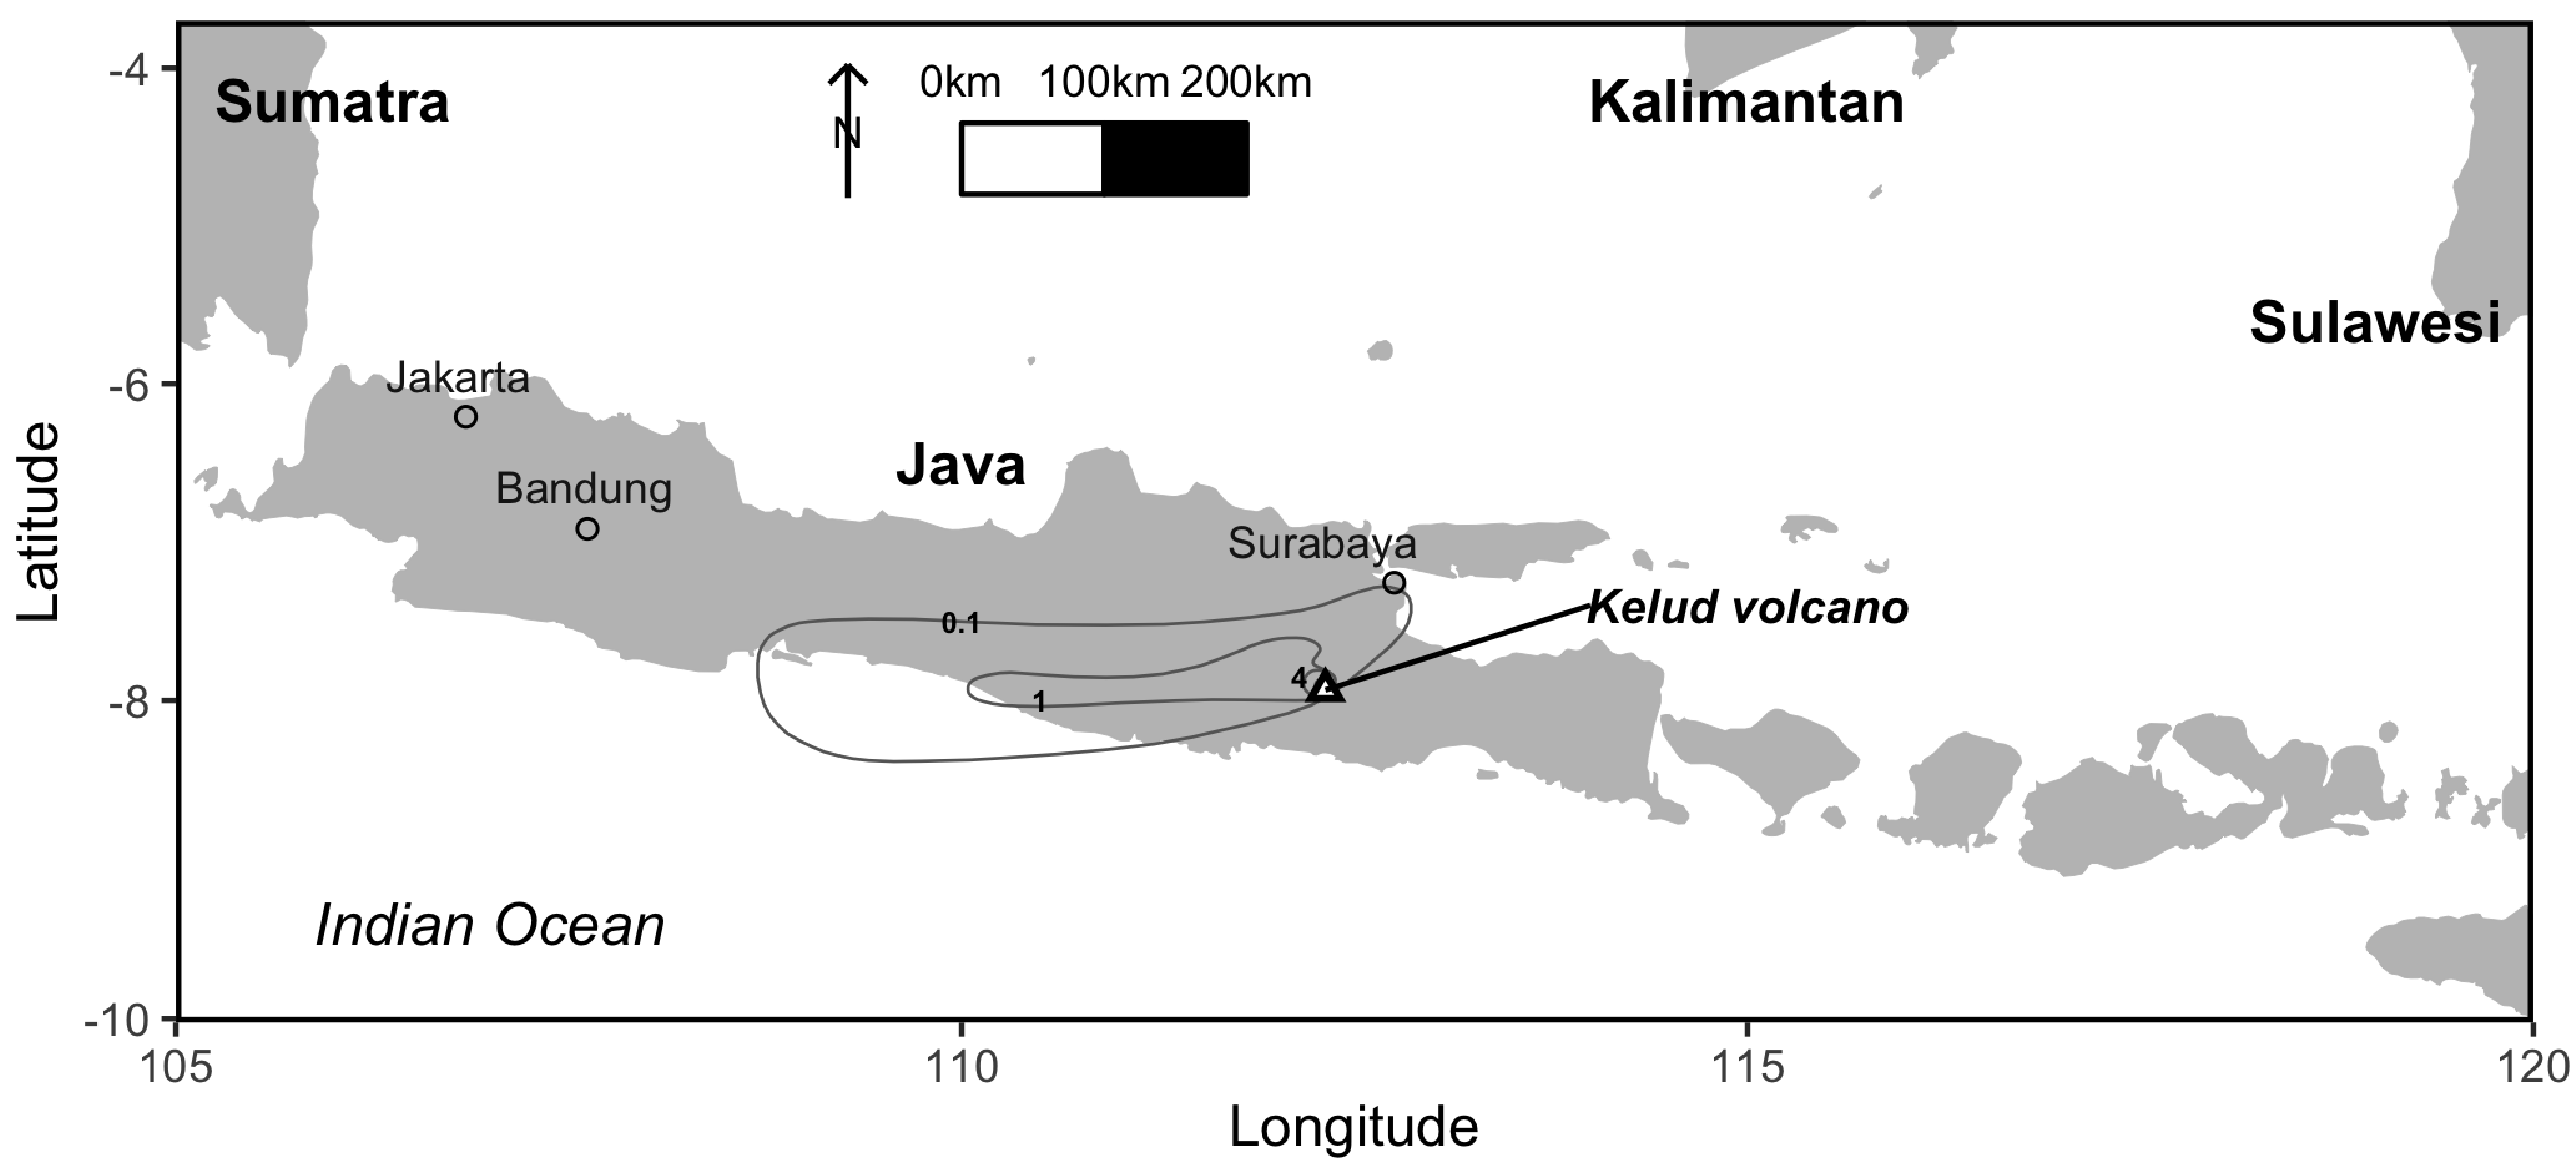
\includegraphics[width=\linewidth]{Figures/fig2_inset-map.png}
\caption{Location map of Kelud volcano in Indonesia. The contours represent tephra thicknesses of 0.1, 1, and 4 cm adopted from \cite{MAENO201924}'s study of the 2014 Kelud eruption fallout deposit.}
\label{fig:insetmap}
\end{figure*}
%%%%%%%%%%%%%%%%%%%%

\subsection{Tephra fall data}\label{subsection-case-data}

The study utilises two sets of tephra fall data, each derived from field surveys by different teams at various times after the eruption. The analysis takes the data in terms of load. When only thickness measurements are available, they are converted to loads based on a deposit bulk density of 1400 $kg/m^{3}$ measured by \cite{MAENO201924}. The first dataset, here called \textit{Dataset 1}, is the tephra load data obtained from a field study of thickness by Universitas Gadjah Mada (UGM) \citep{anggorowati2015} and later used in inversion modelling by \citet{williams2020}. The measurements were taken 2-3 days post-eruption at 81 locations within 2 to 60 km of the vent \citep{williams2020}. The other data set, here called \textit{Dataset 2}, consists of tephra load data converted from thickness measurements from a geological survey by \citet{MAENO201924} conducted a month after the eruption. Dataset 2 provides load information at 50 locations, including areas up to 75km north of the vent that Dataset 1 doesn't cover. For this study, we exclude the six eyewitness reports also presented by \citet{MAENO201924}.

Four outliers were removed from the raw datasets as they were an order of magnitude different than nearby data, potentially related to issues of data collection or significant deposit reworking. Being outside the range of the other observations, these were deemed to have a disproportionately strong influence over the model fits. After removing these outliers, the dataset used in our analyses consists of 127 points. A map of the datasets is presented in Figure \ref{fig:datasets}.


    %%%%%%%%%%%%%%%%%%%%
    \begin{figure*}[htbp]
    \centering
    \includegraphics[width=\linewidth]{Figures/fig3_data.png}
    \caption{Map and histogram of datasets used in the study. The location of Kelud volcano's vent from the 2014 eruption is based on \cite{goode2019insights}'s study of the eruption.}
    \label{fig:datasets}
    \end{figure*}
    %%%%%%%%%%%%%%%%%%%%

\subsection{Previous inversion study}

The value of using inversion and forward estimation with process-based models for Kelud volcano has been presented in recent literature. \cite{williams2020} applied inversion as one of the methods to support remote assessment of tephra fall building damage and vulnerability assessment of buildings around Kelud volcano. In \cite{williams2020}'s study, thickness measurements were inverted to estimate the best-fit source parameters, which were later used to map a continuous deposit. Such application is important to enhance our knowledge of risk to tephra hazards on the the scale of buildings or regions, especially when there is a high likelihood of future damaging eruptions from Kelud \citep{MAENO201924}.


%----------------
\section{Methods}\label{section-methods}
% Provide sufficient detail to allow the work to be reproduced. Methods already published should be indicated by a reference: only relevant modifications should be described. In the case of software papers, the Methods section should include the software design as well as the experimental design for testing the software.
%----------------

\subsection{Model setup for \textit{Tephra2} inversion}\label{subsection-met-setup}

\textit{Tephra2} produces tephra load estimates based on approximations of physical equations for dispersion. The inversions use fixed wind conditions as model inputs. These are expressed as a single wind profile based on the wind dataset from the European Centre for Medium-Range Weather Forecasts (ECMWF) Era-Interim Reanalysis for the midnight of 13 February 2014 \citep{dee2011era}. 

The parameter bounds used in the inversion algorithm are shown in Table \ref{tab:eps}. The ranges of values are selected based on studies in the literature of the 2014 Kelud eruption and a recent inversion for the same eruption in \cite{williams2020}. For this study, some of the ranges of values are widened relative to \cite{williams2020}'s to ensure that the inversion solution converges within the limits set. We use the default optimisation routine from \citet{connor2006inversion}'s inversion algorithm, the Nelder-Mead simplex method.

    %%%%%%%%%%%%%%%
    \begin{table}[]
    \caption{The inversion in this study uses the range of initial values presented in this table. The initial values are selected based on information from: [a] \citet{kristiansen2015stratospheric}, [b] \citet{MAENO201924}, [c] \citet{goode2019insights, MAENO201924}, [d] \citet{goode2019insights, MAENO201924}, and [e] \citet{williams2020}.}
    \label{tab:eps}
    \begin{tabular}{@{}lll@{}}
    \toprule
    Inverted parameters         & 
    Values from literature &
    Initial values for the inversion
     \\ 
    \midrule
    
    Plume height (km above sea level)           &
    18 to 26 [a] &
    15 to 23 
                   \\
    
    Erupted mass $10^{10}$ kg          &
    38 to 66 [b] &
    10 to 100   
                  \\
    
    Median grain size (phi)            & 
    -3 to 1 [c]   &
    -3 to 2.5   
                \\
    
    Phi standard deviation             & 
    1 to 3 [d] &
    0.5 to 3                          
                  \\
    
    Fall-time threshold (s)            & 
    0.001 - 10,000 [e]  &
    0 to 15,000                       
           \\
    
    Diffusion coefficient $(m\,s^{-2})$ & 
    0.0001 - 10,000 [e]  &
    0 to 15,000                       
           \\
    
    Plume profile ($\alpha$)           & 
    3 [e] &
    3                                
            \\
    
    Plume profile ($\beta$)            & 
    0.001 - 3 [e]  &
    0.001 to 3.5                      
           \\ \bottomrule
    \end{tabular}
    \end{table}
    %%%%%%%%%%%%%%%

\subsection{Evaluation of cost function}\label{subsection-met-eval}

In this paper, we consider five cost functions. They consist of functions already in the current \textit{Tephra2} code (i.e., mean square error written as Equation \ref{eq:mse}) and chi-square error as in Equation \ref{eq:chieq}), as well as three additional functions:
\begin{equation}
Mean\;absolute\;error\;(MAE) = \frac{1}{n} \sum_{i=1}^{n} |y_{i} - x_{i}|
\end{equation}
\begin{equation}
Mean\;absolute\;percentage\;error\;(MAPE) = \frac{100}{n} \sum_{i=1}^{n} \left | \frac{y_{i} - x_{i}}{x_{i}} \right|
\end{equation}
\begin{equation}
Mean\;square\;log\;error\;(MSLE) = \frac{1}{n} \sum_{i=1}^{n}\left (log \frac{(y_{i}+1) }{(x_{i}+1)}\right )^2 \label{eq:msleeq}
\end{equation} 
 where $y_{i}$ refers to the model estimate, $x_{i}$ is the observation, and $n$ is the total number of data points.

Instead of Tokyo log error (Equation \ref{eq:tokeq}), this study uses MSLE (Equation \ref{eq:msleeq}), a more well-known cost function in statistics and machine learning. In cases where the observed and predicted values are strictly positive, as in the case of tephra load data, the Tokyo log function is essentially the same as MSLE. In MSLE's formula, the `$+1$'s attached to the observed value $x_{i}$ and predicted value $y_{i}$ ensure mathematical stability since log(0) is undefined and both $y$ and $x$ can be 0. 

We propose a two-step approach to evaluate the choice of cost function for the \textit{Tephra2} inversion. First, the choice should be guided by the properties of the cost function. For instance, some cost functions are more sensitive to outliers, and some are better for data which span orders of magnitude. The properties of the cost functions are summarised in Table \ref{tab:costf} and discussed in Section \ref{subsection-met-prop}, which serves as a guide to narrow down the appropriate cost functions for the test case.

The second step is to run test inversions using the shortlisted cost functions and the set up in Section \ref{subsection-met-setup}, and analyse the resulting residuals. While the choice of the cost function depends on the properties most relevant to the context, it also implies an assumption about the distribution of residuals. MSE, for instance, assumes normally-distributed residuals. Since each cost function is associated with distributional assumptions on the residuals, we can check the suitability of the choice of cost function using goodness-of-fit tests described in Section \ref{subsection-met-fits}. 


\subsubsection{Selection based on cost functions' properties} \label{subsection-met-prop}

    The foundation of any cost function is the model residual, defined as $\varepsilon = y - x$, where $x$ refers to the observed value and $y$ is the predicted value of the model. Cost functions almost always include a transformation of the observed value, predicted value or the residual. This transformation influences the model estimates according to these properties: (1) order-dependence, (2) sensitivity to outliers, and (3) symmetry. The equations for the transformed residuals associated to the cost functions are shown in Table \ref{tab:costf}.
    
    Order-dependence describes how the function covers orders of magnitude for the residual. For instance, an order-dependent cost function may utilise the relative error $\varepsilon / x$ (e.g. in the chi-square cost function) or the log-transform of the observed and predicted values (e.g. in mean square log error, MSLE). On the other hand, a cost function that's not order-dependent, also known as scale-dependent functions, keep the residual $\varepsilon$ as is in the function to retain the units/scale of the observed and modelled values. A comprehensive description of scale-dependent cost functions is provided in \cite{walther2005concepts}. 
    
    If the modeller wishes to balance the treatment of distal and proximal deposits, order-dependent cost functions may be desirable. Since order-dependent cost functions are scaled to the magnitude of the measured value, observations made in thin parts of the deposit are equally important as observations made in the thicker parts of the deposit. This aspect is important due to a few reasons. Tephra deposits thin exponentially with distance from the vent, and outcrops mapped across a single deposit may span orders of magnitude \citep{pyle1989thickness}. Distal measurement of tephra accumulations are important to inform the extrapolation of the thinning rate beyond the outermost isopach. Examples of common order-dependent cost functions include chi-square, MSLE and MAPE.
    
    Some cost functions are more sensitive to outliers than others. Cost functions in which the residual is squared, for instance, penalise large residuals more heavily than small residuals. Common examples are MSE and root-mean-square-error (RMSE), both of which minimise to the same solution. If we prefer to constrain penalty on large errors and make the function more resistant to outliers, the absolute residual $\left |\varepsilon \right |$ can be used instead of $\varepsilon^2$, for instance, with the mean absolute error (MAE). MAE may be more appropriate for instances when the residuals are not normally distributed, when large model residuals don't have to be weighted heavily, and when the presence of outliers is a significant issue. 
    
    Lastly, the symmetry of the cost function relates to the treatment of underestimation versus overestimation. MSE, MAE, and chi-square treat residuals symmetrically. MSLE applies more penalty for underestimation than overestimation. Mean absolute percentage error (MAPE) penalises overestimation more than underestimation. 


\subsubsection{Selection based on cost functions' assumption on residuals} \label{subsection-met-fits}

    The choice of cost function also implies a distribution of residuals. So in addition to their theoretical properties, we can examine the validity of the cost functions by investigating the distribution of resulting residuals using statistical tests such as the Kolmogorov-Smirnov (K-S), the Cram{\'e}r-von-Mises (CvM) and the Anderson-Darling (A-D) as well as the Shapiro-Wilk (S-W) \citep{Kandethody2015, Stephen1986}. These tests use different metrics or test statistics to measure how similar the empirical distribution of the residuals is to its assumed one. For example, the K-S test statistic is:
    \begin{equation}
        D = \max(|F_{0}(\epsilon) - F_{n}(\epsilon)|),
    \end{equation}
    where $F_{0}(\epsilon)$ is the assumed cumulative distribution function and $F_{n}(\epsilon)$ is the empirical cumulative distribution of the residuals. The larger $D$ is, the more unlikely the residuals to have been generated from the assumed distribution. Goodness-of-fit can also be assessed graphically using quantile-quantile (Q-Q) plots which compare the empirical quantiles from the model fit to the theoretical quantiles from their assumed distributions. While both statistical tests and Q-Q plots are useful indicators of goodness-of-fit, they both assume that the residuals are themselves independent and identically distributed. 


\afterpage{%
    \clearpage% Flush earlier floats (otherwise order might not be correct)
    \begin{landscape}% Landscape page
    \centering % Center table
    %%%%%%%%%%%%%%%%
    \begin{table}[]
    % \scriptsize
    \caption{Cost functions with their formulae, residual transformation and assumed error distributions. In the formulae, $x$ refers to the observation, $y$ the model estimate, $n$ the number of data points and $\varepsilon = y-x$ the residual. For the Gaussian distributions, $\hat{\sigma}$ denotes the estimated standard deviation, while for the Laplace distributions, $b$ denotes the estimated scale. Characteristics of the cost functions are provided with a recommendation of when these are useful for tephra load inversion. The checkmarks indicate if the cost function satisfies a specific characteristic.}
     \label{tab:costf}
    \begin{tabular}{@{}lcccccc@{}}
    \toprule
    \multicolumn{1}{c}{\multirow{2}{*}{}} 
    & \multirow{2}{*}{}                                                 
    & \multicolumn{5}{c}{Cost function}                                    \\ \cmidrule(l){3-7} 
    \multicolumn{2}{c}{}                                                                                                                        & MSE                                                                  & MAE                                                                  & Chi-square                                                           & MSLE                                                                 & MAPE                                                                 \\ \midrule
    \multicolumn{2}{c}{\textbf{Formula}}                                    & $\frac{1}{n} \sum_{i=1}^{n} \varepsilon_{i}^{2} $ & $\frac{1}{n} \sum_{i=1}^{n} \left |\varepsilon_{i} \right |$ & $\frac{1}{n} \sum_{i=1}^{n} (\varepsilon_{i}^2 / x)$ & $\frac{1}{n} \sum_{i=1}^{n} \left (log \frac{(y_{i}+1) }{(x_{i}+1)} \right )^2$ & $\frac{100}{n} \sum_{i=1}^{n} \left | \frac{\varepsilon_{i}}{x_{i}} \right |$ \\ \midrule
    \multicolumn{2}{c}{ \textbf{Transformed residual} $Z_{i}$}            & $Predicted - Actual$                                                 & $Predicted - Actual$                                                 & $\frac{Predicted - Actual}{\sqrt{Actual}}$                           & $\log_{10}\left(\frac{Predicted + 1}{Actual + 1}\right)$             & $\frac{Predicted - Actual}{Actual}$                                  \\ \midrule
    \multicolumn{2}{c}{\textbf{Assumed distribution}}                                                           & $\frac{Z_{i}}{\hat{\sigma}} \sim N(0, 1)$                                                    & $\frac{Z_{i}}{\hat{b}} \sim Laplace(0, 1)$                                                        & $\frac{Z_{i}}{\hat{\sigma}} \sim N(0, 1)$                                                      & $\frac{Z_{i}}{\hat{\sigma}} \sim N(0, 1)$                                                                   & $\frac{Z_{i}}{\hat{b}} \sim Laplace(0, 1)$                                                                          \\ \midrule
    \multicolumn{2}{c}{\textbf{Scale-dependent}} & \multicolumn{5}{l}{The units of the observed and predicted values are retained. Useful for interpretability
    .}      \\
    \multicolumn{2}{c}{\textbf{}} & $\checkmark$                                                          & $\checkmark$                                                                     &                                                                          &                                                                                                     &                                                                                                   \\ %\midrule
    \multicolumn{2}{c}{\textbf{Order-dependent}} & \multicolumn{5}{l}{Thinner deposits are as important as thicker deposits. Useful when spanning orders of magnitude.} \\
    \multicolumn{2}{c}{\textbf{}}                                                                   &    &                                                                                  & $\checkmark$                                                             & $\checkmark$                                                                                        & $\checkmark$                                                                                      \\ \midrule
    \multicolumn{2}{c}{\textbf{Sensitive to outliers}} & \multicolumn{5}{l}{Estimates fit large values closely. Useful when these are the most reliable and informative.} \\
    \multicolumn{2}{c}{\textbf{}} & $\checkmark$                                                          &                                                                                  &   $\checkmark$                                                                       &                                                                                                     & $\checkmark$                                                                                      \\ %\midrule
    \multicolumn{2}{c}{\textbf{Robust against outliers}} & \multicolumn{5}{l}{Reduced penalty on large residuals. Useful when there are many outliers in the data.} \\
    \multicolumn{2}{c}{\textbf{}}       &       & $\checkmark$                                                                     &                                                              & $\checkmark$                                                                                        &                                                                              \\ \midrule
    \multicolumn{2}{c}{\textbf{Symmetric}} & \multicolumn{5}{l}{Treats overestimation and underestimation equally. Useful to avoid anomalous skewness in errors.} \\
    \multicolumn{2}{c}{\textbf{}} & $\checkmark$                                                          & $\checkmark$                                                                     & $\checkmark$                                                             &                                                                                                     &                                                                            \\ %\midrule
    \multicolumn{2}{c}{\textbf{Asymmetric}} & \multicolumn{5}{l}{Treats overestimation and underestimation unequally. Useful for avoiding either scenario.} \\
    \multicolumn{2}{c}{\textbf{}} & \multicolumn{1}{l}{}                                                  &                                                             & \multicolumn{1}{l}{}                                                     & $\checkmark$*                         & $\checkmark$**              \\ \bottomrule
    \multicolumn{7}{l}{*Larger penalty for underestimation. **Much larger penalty for overestimation.}
    \end{tabular}
    \end{table}
    %%%%%%%%%%%%%%%%
\end{landscape}
\clearpage% Flush page
}

\subsection{Weighting the data in the cost function} \label{subsection-met-weight}

In order to account for different levels of uncertainty inherent in our datasets, we propose to weigh each data point based on its uncertainty relative to a reference dataset. In this way, less reliable data have correspondingly less influence on the inversion. The reference dataset may be an individual measurement or a group of measurements having the least measurement uncertainty. In this work, we use the prior information that Dataset 2 has a relatively larger uncertainty than Dataset 1 because of the delay in field data acquisition between the two sets of data. Thus, Dataset 1 is set as the reference dataset. In the inversion algorithm, points in this reference dataset are assigned a weight of 1. Other datasets are then assigned weights relative to the uncertainty of the reference data. For example, the points from a dataset assumed to be twice as uncertain as the reference dataset may be assigned a weight, $w$, of 0.5. 

Using weights based on relative uncertainty leads to a weighted cost function, where each data point is weighted relative to the reference dataset. With our proposed weighting scheme, the weighted MSE cost function, for instance, can be written as:
\begin{equation}
\frac{1}{n} \sum_{i=1}^{n} w_{i} (y_{i} - x_{i})^{2}
\end{equation}
where $w_{i}$ indicates the uncertainty weight assigned to the data point $i$. For our application, we set Dataset 2's weight to 0.5. 

We evaluate the effectiveness of the weighted cost function based on the accuracy of the forward estimates on unseen (out-of-sample) data. The test set consists of a random subset (20\%) of Dataset 1, while the training set consists of the rest of the Dataset 1 points and all of Dataset 2 (Figure \ref{fig:train-test}). A test set should ideally consist of data that closely resembles the true deposit, so a stratified test set was selected to represent thin and thick deposits in relatively equal proportion as the true deposit. Inversion is conducted using the training points, the parameter ranges in Table \ref{tab:eps}, and the weighted form of the cost function. For all the inversions, we generate forward estimates of tephra load on the locations of the test points. To assess predictive performance, we compare the test errors between the unweighted inversion and weighted inversion. The test errors are calculated following the formula of the cost function used in the inversion.

    %%%%%%%%%%%%%%%%%%%%
    \begin{figure*}[htbp]
    \centering
    \includegraphics[width=.9\linewidth]{Figures/fig4_train-test.png}
    \caption{The effectiveness of the weighted cost function was evaluated using a train-test split process. Shown is a map of the training and test points used for the methods in Section \ref{subsection-met-weight}.}
    \label{fig:train-test}
    \end{figure*}
    %%%%%%%%%%%%%%%%%%%%

\subsection{Combining model estimates and data} 
\label{subsection-kriging}

To estimate the spatial distribution of tephra load across the entire area, we propose to combine both forward model estimates as well as the data. The process consists of three general steps: (1) calculate the residuals between the forward model and data, (2) interpolate these residuals using spatial statistics techniques, and (3) combine the interpolated residuals with the forward model. Before performing the interpolation, the model residuals can be transformed to an appropriate form as suggested by any of the formulas for $Z_{i}$ in Table \ref{tab:costf}. We test and present two different spatial statistics techniques for the interpolation step. The result is an improved estimate of tephra load that combines the information of the model and data. We elaborate on the process in this section. 

Our methods use kriging, one of many interpolation techniques that estimate values at unobserved locations using a limited set of known spatial data. In kriging, the interpolation accounts for the spatial arrangement of the data in such a way that points nearby the site of interest are given more weight than those farther away. This approach differs from another popular method, inverse distance weighted interpolation, in that we do not assume a spatial distribution model beforehand but estimate it from data. Another advantage of kriging is that we can estimate the uncertainty associated with the interpolated value. 

\subsubsection{Unweighted model-data fusion} \label{subsection-kriging-interp}

We describe the procedure for an \textit{unweighted} model-data fusion approach via kriging. The approach is unweighted as it doesn't account for any differential uncertainty between individual or groups of data. In the methods that follow, we adopt simple kriging, which assumes that the difference between model and data all over the study area has a mean of zero and follow a multivariate normal distribution  \citep{Wackernagel2003}. Peforming kriging involves choosing a \textit{variogram model} and checking the adequacy of the assumptions by the model. The variogram model defines the spatial relationship between each pair of points in the data. Mathematically, it relates the degree of variation in the sampled values and the spatial distance between these points. The parameters of the variogram model are typically user-defined or fitted with statistical software that uses approaches like maximum likelihood and least-squares estimation. Typically, we assume that the variogram and hence the distribution of the residuals is stationary and isotropic. This means that the characteristics of the distribution, particularly how the correlation decreases with pairwise distance, do not change with the location or direction.


\begin{enumerate}

    \item 
    Calculate residuals $Z_{i}$ (from Table \ref{tab:costf}) between the best-fit modelled output and data:
    
    \begin{enumerate}
        \item
        Run the inversion following Section \ref{subsection-met-setup} to find the best-fit parameters. For the calibration of parameters, use the most appropriate cost function identified using the steps in Section \ref{subsection-met-eval}.
    
        \item 
        Using \textit{Tephra2} and the best-fit parameters, estimate the load of tephra fall at all sites (sampled and unsampled).
    \end{enumerate}

    \item 
    Interpolate the residuals using kriging:
    
    \begin{enumerate}
    \item
    For the sampled sites, calculate the residuals using the equations for $Z_{i}$ in Table \ref{tab:costf} that corresponds to the cost function used in Step 1a.
    
    \item 
    Conduct a simple kriging interpolation to predict the residuals at all sites (sampled and unsampled sites) in the study area. The residual at any prediction location $s_{o}$ can be calculated as:
    \begin{equation} \label{eq:simpkrigz}
    \hat{Z}(s_{o}) = \sum_{i=1}^{N} \lambda_{i} Z(s_{i}) 
    \end{equation} 
    where $Z(s_{i})$ is the residual at an observed location $s_{i}$, $\lambda_{i}$ is the kriging weight applied to the value at the observed location, and $N$ is the number of observed sites. The kriging weights $\lambda_{i}$ are calculated from a variogram model and a covariance matrix $\Sigma$, which describes the spatial relationships among the values at the observed sites and the prediction location. The Appendix (\ref{supp-c}) provides a step-by-step procedure for simple kriging interpolation that includes formulas for $\lambda_{i}$ and the covariance matrix $\Sigma$.
    \end{enumerate}
    
    \item 
    Combine the best-fit modelled output and the interpolated residuals:
    
    \begin{enumerate}
    \item
    Back-transform the kriging predictions $\hat{Z}(s_{o})$ to produce residuals with the same units as the data (See the Appendix \ref{supp-c-back} for sample formulas to use when back-transforming the kriging predictions).
     
    \item
    For all locations in the study area, add the estimates of tephra load from Step 1b to the back-transformed residuals from Step 3a. This produces an updated map of tephra fallout that accounts for both the model and the observations.
        
    \end{enumerate}
    
    
    
\end{enumerate}


\subsubsection{Weighted model-data fusion} \label{subsection-kriging-worden}

    In practice, we could have different amounts of uncertainty associated with different datasets collected, as we do in our case study due to different survey teams measuring tephra load at different time points after the eruption. To account for varying data uncertainty in the interpolation procedure presented in Section \ref{subsection-kriging-interp}, we can use an extension of simple kriging introduced by \cite{worden2018}, which they use in the context of earthquake ground motion intensity estimation. The method starts by identifying a \textit{reference dataset} - a subset of the data with least uncertainty. Then, we define the additional uncertainty associated with other datasets relative to this reference dataset.
  
    For the Kelud test case, we set Dataset 1 as the reference dataset because it was acquired the earliest after the eruption. We can set an uncertainty weight of $w_{k=1} = 1$ for Dataset 1 and $w_{k=2} = 0.5$ for Dataset 2. More generally, for datasets other than the reference dataset (Dataset $k > 1$), we will always have $w_{k}$ < 1. Based on these uncertainty weights, we can define an adjustment factor that relates the variance of the reference dataset to other datasets (Dataset $k > 1$) as $a_{k} = \sqrt{w_{k}}$.
  
    The procedure follows the same steps as in Section \ref{subsection-kriging-interp} except for Step 2b. With an adjustment factor, the equation for the residual at any prediction location (originally Equation \ref{eq:simpkrigz}) would become:
        \begin{equation} \label{eq:simpkrig-z2}
        \hat{Z}(s_{o}) = \sum_{i=1}^{N} \lambda^{'}_{i} a_{k} Z(s_{i,k})
        \end{equation} 
    where $Z(s_{i,k})$ is the residual at observation site $i$ and associated with dataset $k$. The adjusted kriging weight, $\lambda^{'}_{i}$, is calculated based on an adjusted covariance matrix $\Sigma'$. The adjusted covariance matrix can be written as:
        \begin{equation} \label{eq:covadjust}
        \Sigma' = \Omega \odot \Sigma
        \end{equation} 
    where $\Omega = \mathbf{a}\mathbf{a}^{T}$, $\mathbf{a}$ is the vector of adjustment factors corresponding to the observation sites ${s}_{1}, \dots {s}_{N}$, and $\odot$ denotes the element-wise multiplication. Note that the covariance matrix and variogram model parameters were estimated using the reference dataset only. 
  
    Similar to the simple kriging approach in Section \ref{subsection-kriging-interp}, we can estimate the uncertainty associated with the interpolated values. Also following Steps 3a and 3b in Section \ref{subsection-kriging-interp}, we can add the interpolated residuals to the optimised model estimates. The result is an updated map of the tephra load that accounts for the model estimates, the observations, and the varying uncertainty between different sets of data.

\subsubsection{Comparison of the kriging methods}
  
    We assess the performance of the kriging methods in Section \ref{subsection-kriging-interp} and \ref{subsection-kriging-worden} using leave-one-out cross-validation (LOOCV). Cross-validation is a popular method to compare the test performance between models. The total number of points used for testing is maximised via iterative sampling and model fitting. LOOCV is a type of cross-validation where just a single observation is held out for testing in every iteration; thus estimating the out-of-sample estimation performance \citep{shao1993linear}. 
    
    We can also check if the kriging interpolation overfits the training points. To confirm this, we compare the LOOCV errors to pre-kriging training errors calculated using the same performance metrics (root mean square error, chi-square, and mean square log error) from the process-based model fit. Since in LOOCV we are conducting out-of-sample estimation, LOOCV errors which are higher than the training errors from the \textit{Tephra2} fit would suggest that kriging overfits the data.
  
%----------------
\section{Results and Discussion}\label{section-results} % or results and discussion
% Results should be clear and concise. In the case of software papers, results should provide both the implementation of the software and the results of the experimental test cases.
%----------------

The study shows that there is a significant influence on the inversion results and forward spatial estimates due to (1) the choice of the cost function in inversion, (2) the treatment and accounting of differential uncertainty of the data, and (3) the treatment and accounting of the spatial characteristics of the data. In the following subsections, we detail these in turn.

%%%%%%%%%%%%%%%%%%%%%%
\subsection{Use of a suitable cost function} \label{subsection-res-costf}
%%%%%%%%%%%%%%%%%%%%%% 

In order to identify the characteristics of cost functions most applicable to the test case, we assessed the distribution of data values and the presence of outliers. The data cover a wide range of values (near zero to 168 $kg/m^{2}$, see Figures \ref{fig:datasets}C and \ref{fig:datasets}D) so we select an order-dependent cost function for a balanced treatment of data across different orders of magnitude. We also decided to use a cost function that is not sensitive to outliers because of the presence of relatively few large values located close to the vent. Using Table \ref{tab:costf} as a guide, the cost functions that satisfy such characteristics are MSLE and chi-square.

Although MAPE is also order-dependent, and most interpretable among all the cost functions in Table \ref{tab:costf} (because the errors it produces are in terms of percentages), we identify it as inappropriate for the test case for reasons beyond its sensitivity to outliers. The Statistics literature has provided evidence of its numerous weaknesses as a cost function. When MAPE is used for optimisation, estimated values become consistently low \citep{tofallis2015better}. Small actual values (less than one) result to extremely large MAPEs, while zero actual values yields infinite errors \citep{kim2016new}. Numerous small data are observed in the test case, which is a common occurrence in tephra fallout data. We also provide a short summary of issues associated with MAPE in the Supplementary Information.

Between MSLE and chi-square, MSLE is identified as the more suitable cost function because the residuals associated to the inversion with MSLE best adhered to the cost function's statistical assumption. This was demonstrated with MSLE giving the largest p-values across all the goodness-of-fit tests in Table \ref{tab:GOF_loss}. The Q-Q plots in Figure \ref{fig:gaussian_qq} also support the conclusion because the matched theoretical and empirical quantiles lie along the diagonal line for MSLE. The Q-Q plots for the cost functions with underlying Laplace distributions (MAE and MAPE) are given in the Supplementary Information.

    %%%%%%%%%%%%%%%%%%%
    \begin{table}[tbp]
    \centering
    \caption{Goodness-of-fit tests for different cost functions. The null hypotheses for the Kolmogorov-Smirnov (K-S), the Cram{\'e}r-von-Mises (CvM), the Anderson-Darling (A-D) and the Shapiro-Wilk (S-W) tests are that the residuals follow the assumed distributions. So, large p-values indicate better adherence to the assumptions. For our tephra case study, the residuals from the MSLE model fit seem to fit its assumed distribution the best. The Shapiro-Wilk test is only applicable for Gaussian distributions, thus, inapplicable for cost functions with underlying Laplace distributions, such as MAE and MAPE.}
    \begin{tabular}{lllll}
    \hline
    \multirow{2}{*}{Cost function} &  K-S statistic & CvM statistic & AD statistic & S-W statistic \\
    & (p-value) & (p-value) & (p-value) & (p-value) \\
    \hline
    \multirow{2}{*}{MSE}  & 0.155 & 0.285 & 1.684	& 0.937 \\
     & (0.082) & (0.149) & (0.138) & (0.003) \\
    \hline
    \multirow{2}{*}{chi-square}    & 0.216 & 0.966 & 4.728 & 0.948 \\
     & (0.004) & (0.003) & (0.004) & (0.009) \\
    \hline
    \multirow{2}{*}{\textbf{MSLE}}  & 0.060 & 0.039 & 0.327 & 0.916 \\
    & \textbf{(0.967)} & \textbf{(0.938)} & \textbf{(0.916)} & \textbf{(0.205)} \\
    \hline
    \multirow{2}{*}{MAE}  &   0.156 & 0.243 & 1.520 & not applicable \\
     & (0.079) & (0.198) & (0.172) &  \\   
    \hline
    \multirow{2}{*}{MAPE}  & 0.245 & 1.264 & 6.003 & not applicable \\
    & (0.001) & (0.001) & (0.001) &  \\ 
    \hline
    \end{tabular}
    \vspace{2mm}
    \label{tab:GOF_loss}
    \end{table}
    %%%%%%%%%%%%%%%%%%%

    %%%%%%%%%%%%%%%%%%%
    \begin{figure}[tbp]
    \centering
    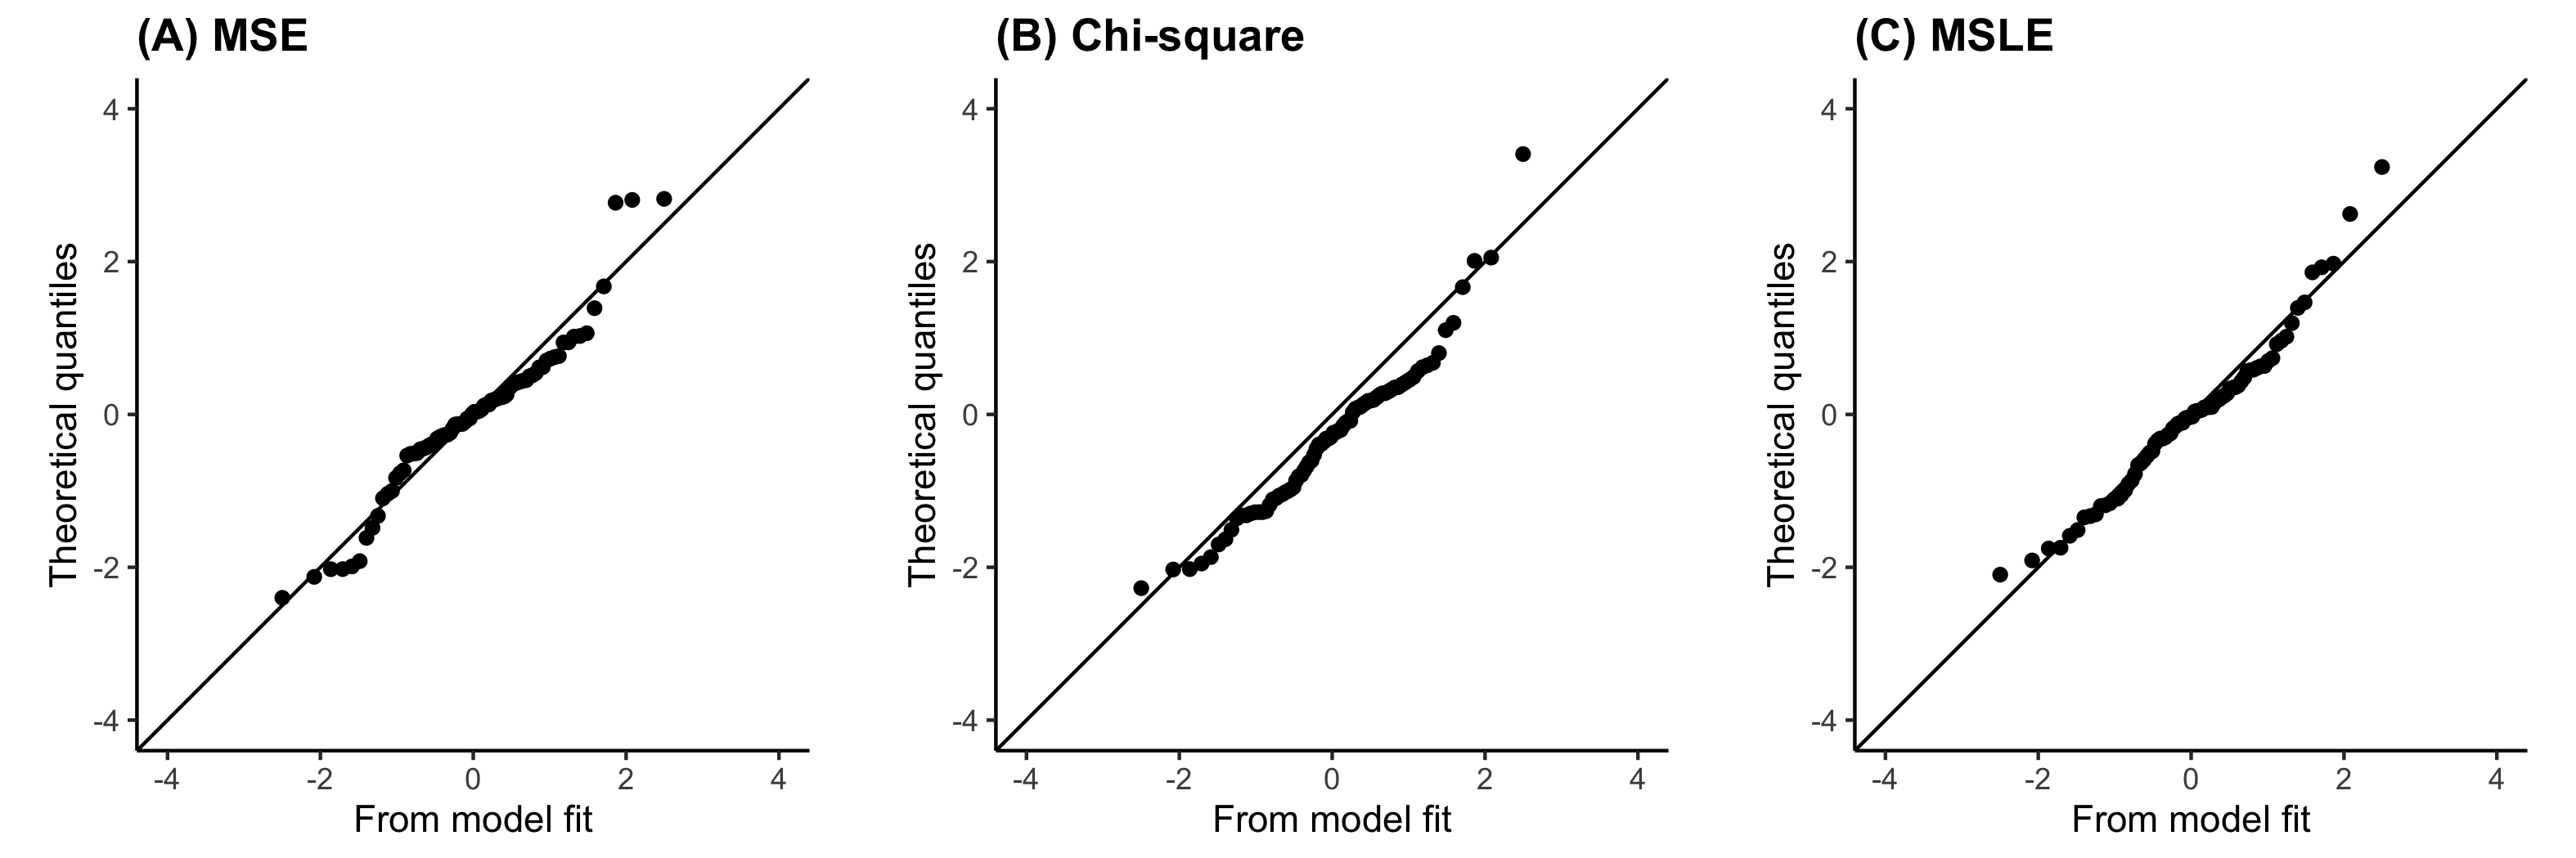
\includegraphics[width=\linewidth]{Figures/fig5_qq-plots.png}
    \caption{Quantile-quantile (Q-Q) plots illustrating goodness-of-fit for the models fitted using different cost functions: MSE, chi-square loss and MSLE. The fit is evaluated by how well the empirical quantiles from the transformed model residuals line up with the theoretical quantiles from the assumed distributions along the diagonal line.}
    \label{fig:gaussian_qq}
    \end{figure}
    %%%%%%%%%%%%%%%%%%%

In summary, while little attention is usually given to the choice of the cost function in the inversion of source parameters, our analyses highlight that the selection of cost function needs to be a conscious choice since each has associated assumptions on how the model would fit the data. Results in Figure \ref{fig:gaussian_qq} show that using different cost functions can have a strong influence on the residuals of the best-fit modelled output. More importantly, residual analysis can be used to draw conclusions on the appropriateness of the selected cost function. Using the methods presented, We found that MSLE performs well and has characteristics well-suited for the case study. 

%%%%%%%%%%%%%%%%%%%%%%
\subsection{Weighting the cost function based on varying uncertainty} \label{subsection-varuncert}
%%%%%%%%%%%%%%%%%%%%%%

The purpose of adding uncertainty-based weights to the cost function in the inversion is to fit the model to the more reliable data, while still considering the information provided by other less reliable data. In the test case, Dataset 2 is the less reliable dataset compared to Dataset 1; nevertheless, Dataset 2 is important to consider as it provides information in the deposit that might not be captured by Dataset 1. For instance, only Dataset 2 consists of load data that are less than 1 kg$/m^{2}$. These relatively small measurements are located in areas north and south of the vent where Dataset 1 does not cover (Figure \ref{fig:datasets}). 

The improved fit to the more reliable data can be visualised by looking at how the distribution of residuals change when using a weighted inversion versus those of an unweighted inversion. For the test case's weighted inversion, the residuals at the locations of the reference dataset (Dataset 1) became more concentrated around zero compared to those of the unweighted inversion (Figure \ref{fig:histvaruncert}A). This difference in the distributions in Figure \ref{fig:histvaruncert}A indicate that the weighted inversion was successful in terms of fitting better to the reference dataset. As expected, the distribution of residuals for Dataset 2 from the weighted inversion does not indicate an improved fit (Figure \ref{fig:histvaruncert}B). The residual distribution for Dataset 2 only show a subtle increase in positive residuals when the inversion was weighted.

 %%%%%%%%%%%%%%%%%%%%%
    \begin{figure*}[htbp!]
    \centering
    \includegraphics[width=\linewidth]{Figures/fig6_histograms-weighting.png}
    \caption{A visualisation of improving the fit to the more reliable dataset (Dataset 1) through a weighted inversion. Shown are histograms of residuals for inversions that make use of an unweighted and weighted MSLE cost function. Shown in (A) are residuals at locations of Dataset 1, whereas (B) shows the residuals at Dataset 2 locations.}
    \label{fig:histvaruncert}
    \end{figure*}
    %%%%%%%%%%%%%%%%%%%%%

We assessed how uncertainty-based weights in the cost function impact the best-fit modelled output of an inversion-forward estimation analysis for tephra fallout. Following the method in Section \ref{subsection-met-weight}, we conducted the inversion using MSLE, the cost function that worked best based on the results in Section \ref{subsection-res-costf}. Since the selected cost function was MSLE, the test errors were calculated using the MSLE formula (Equation \ref{eq:msleeq}). When no weights were applied to the training points, the test error is 0.05, whereas, with weights applied, the test error is 0.03 (Table \ref{tab:test-errors}). Using weights in the inversion resulted in a lower test error, which implies that using weights resulted in a better predictive performance at out-of-sample locations. We checked whether using different cost functions would result in the same behaviour. Thus, we repeated the inversions using the same train-test split, uncertainty weights, and initial parameter ranges but using cost functions other than MSLE. The resulting test errors, shown in Table \ref{tab:test-errors}, indicate that using weights in the inversion consistently reduces test errors, and thus improves the prediction capability of the inversion-forward estimation analysis.


    %%%%%%%%%%%%%%%%%%%%%%%%
    % Please add the following required packages to your document preamble:
    % \usepackage{multirow}
    \begin{table}[htbp]
    \centering
    \caption{Multiple inversions were conducted using the same training points (see train-test split in Figure \ref{fig:train-test}) and initial parameter ranges (Table \ref{tab:eps}), but using different cost functions. The first set of inversions was run with no uncertainty-based weights applied to the training points. Shown in column (a) are the resulting errors at the test points calculated in the units of the corresponding cost function used in the calibration. Column (b), on the other hand, has weights applied to the training points in the inversion. The test errors show that applying weights results in a consistent decrease in the test errors leading to better predictive performance.}
    \label{tab:test-errors}
    \begin{tabular}{ccc}
    \hline
    \multicolumn{1}{l}{\multirow{2}{*}{\begin{tabular}[c]{@{}l@{}}Cost function used\\ in the calibration\end{tabular}}} & \multicolumn{2}{c}{Test errors}\\ \cline{2-3} 
    \multicolumn{1}{l}{} & \begin{tabular}[c]{@{}c@{}} (a) No weights applied\\ to training points\end{tabular} & \begin{tabular}[c]{@{}c@{}} (b) Weights applied\\ to training points\end{tabular} \\ \hline
    MSE & 123.4   & 109.6   \\
    MAE & 8.77  & 8.75  \\
    Chi-square   & 106.1   & 97.5   \\
    MSLE    & 0.05  & 0.03    \\
    MAPE   & 68.5    & 67.1   \\ \hline
    \end{tabular}
    \end{table}
    %%%%%%%%%%%%%%%%%%%%%%%%

%%%%%%%%%%%%%%%%%%%%%%
\subsection{Influence on the source parameters} \label{subsection-res-params}
%%%%%%%%%%%%%%%%%%%%%%

Thus far, the presented methodological contributions on the inversion (use of appropriate cost functions, and applying weights to the cost function) were investigated in terms of their impacts on the best-fit modelled outputs and the associated residuals. Acknowledging that the primary focus of an inversion is to optimise for the best-fit source parameters, we summarise the best-fit parameter values from inversions using different cost functions in Table \ref{tab:esps_costf} and for different weighting schemes in Table \ref{tab:esps_wt}. The purpose of the paper is to not make claims about the true source parameters for the test case, instead we highlight that the source parameters are sensitive to the cost function and weighting in the inversion. 

In Section \ref{subsection-res-costf}, we discuss how the order-dependence and outlier-sensitivity properties of cost functions may influence the model fit to large (often proximal to the vent) and small values (often distal).In Section \ref{subsection-varuncert}, the weighted approach allows a better fit to the more reliable data, no matter the data's magnitude. The relationship of the source parameters to these characteristics, i.e. the estimation of thicker deposits near the vent or thinner distal deposits, is affected by the physics of tephra transport. For instance, a larger plume height may lead to more tephra deposition at distal sites due to tephra being dispersed farther downwind, while a lower plume height may lead to thicker proximal deposit because of less wind advection. The relationship of observations made in distal and proximal sites to source parameters such as the erupted mass and plume height parameters have been studied by \citet{suzuki1983theoretical}, \cite{bonadonna2005probabilistic}, and \cite{yang2021tephra}.

A full understanding of the sensitivity of the proposed methods to each source parameter would require more extensive sensitivity analyses and preferably a test case with a bigger dataset. Parameter sampling algorithms, such as Markov Chain Monte Carlo algorithms, are popular for evaluating the benefits of new inversion methods (e.g. \cite{white2017efficient, yang2021tephra}). Such methods may run the inversion thousands of times using different starting seeds to produce a range of fitted parameter values. The algorithms can extract confidence intervals for the source parameters, which can represent the impact of the new methods on the optimised parameters. While such sensitivity analysis is out of scope of this paper, our analysis highlights the importance of cost function selection and weighted inversion when varying data uncertainties are present when such studies are implemented. In this way, our work can contribute towards improving our understanding of relationships between data uncertainty and source parameters in the inversion.


\afterpage{%
    \clearpage% Flush earlier floats (otherwise order might not be correct)
    \begin{landscape}% Landscape page

% Please add the following required packages to your document preamble:
% \usepackage{multirow}
\begin{table}[]
\centering
\caption{Best-fit parameter values from inversions using different cost functions. All inversions used unweighted cost functions, Dataset 1 for training, and the range of parameter values in Table \ref{tab:eps} (asl = above sea level).}
\label{tab:esps_costf}
\begin{tabular}{crrrrrrrr}
\hline
\multirow{2}{*}{\begin{tabular}[c]{@{}c@{}}Cost function\\ (no weights applied\\ to training points)\end{tabular}} & \multicolumn{8}{c}{Inverted parameters' best-fit value} \\ \cline{2-9} & \multicolumn{1}{c}{\begin{tabular}[c]{@{}c@{}}Column\\ height\\ (km asl)\end{tabular}} & \multicolumn{1}{c}{\begin{tabular}[c]{@{}c@{}}Erupted\\ mass\\ ($10^{10}$ kg)\end{tabular}} & \multicolumn{1}{c}{\begin{tabular}[c]{@{}c@{}}Grain size\\ Median\end{tabular}} & \multicolumn{1}{c}{\begin{tabular}[c]{@{}c@{}}Grain size\\ standard\\ deviation\end{tabular}} & \multicolumn{1}{c}{\begin{tabular}[c]{@{}c@{}}Fall time\\ threshold\\ ($s$)\end{tabular}} & \multicolumn{1}{c}{\begin{tabular}[c]{@{}c@{}}Diffusion\\ coefficient\\ (m $s^{-2}$)\end{tabular}} & \multicolumn{1}{c}{\begin{tabular}[c]{@{}c@{}}Plume\\ profile,\\ $\alpha$\end{tabular}} & \multicolumn{1}{c}{\begin{tabular}[c]{@{}c@{}}Plume\\ profile,\\ $\beta$\end{tabular}} \\ \hline
MSE   & 23.3    & 87.7    & 1.24    & 1.37   & 6356  & 10221   & 3  & 3.38     \\
MAE  & 22.3   & 66.5  & 0.79     & 0.58   & 14380  & 10288    & 3    & 3.38    \\
Chi-square    & 23.6   & 89.9  & 1.87   & 2.15  & 1406   & 12116  & 3  & 2.92  \\ 
MSLE   & 17.4   & 67.7   & 0.85   & 1.06   & 2070   & 14748  & 3   & 1.30   \\
MAPE   & 24.0  & 57.8   & 1.03    & 1.27    & 4937    & 5389   & 3  & 2.98  \\ \hline
\end{tabular}
\end{table}
\end{landscape}
\clearpage% Flush page
}

\afterpage{%
    \clearpage% Flush earlier floats (otherwise order might not be correct)
    \begin{landscape}% Landscape page

% Please add the following required packages to your document preamble:
% \usepackage{multirow}
\begin{table}[]
    \centering
\caption{Best-fit parameter values from inversions using different cost functions. All inversions make use of Dataset 1 and 2 for training. The range of parameter values in Table \ref{tab:eps} were used to initiate the inversions. The weighted cost functions follow the procedure in Section \ref{subsection-met-weight}. (asl = above sea level)}
\label{tab:esps_wt}
\begin{tabular}{crrrrrrrr}
\hline
\multirow{2}{*}{\begin{tabular}[c]{@{}c@{}}Cost function\\ and associated\\ weighting scheme\end{tabular}} & \multicolumn{8}{c}{Inverted parameters' best-fit value}   \\ \cline{2-9}  & \multicolumn{1}{c}{\begin{tabular}[c]{@{}c@{}}Column\\ height\\ (km asl)\end{tabular}} & \multicolumn{1}{c}{\begin{tabular}[c]{@{}c@{}}Erupted\\ mass\\ ($10^{10}$ kg)\end{tabular}} & \multicolumn{1}{c}{\begin{tabular}[c]{@{}c@{}}Grain size\\ Median ($\phi$)\end{tabular}} & \multicolumn{1}{c}{\begin{tabular}[c]{@{}c@{}}Grain size\\ standard\\ deviation ($\phi$) \end{tabular}} & \multicolumn{1}{c}{\begin{tabular}[c]{@{}c@{}}Fall time\\ threshold\\ ($s$)\end{tabular}} & \multicolumn{1}{c}{\begin{tabular}[c]{@{}c@{}}Diffusion\\ coefficient\\ (m $s^{-2}$)\end{tabular}} & \multicolumn{1}{c}{\begin{tabular}[c]{@{}c@{}}Plume\\ profile,\\ $\alpha$\end{tabular}} & \multicolumn{1}{c}{\begin{tabular}[c]{@{}c@{}}Plume\\ profile,\\ $\beta$\end{tabular}} \\ \hline
\multicolumn{9}{l}{\textbf{MSE}}  \\
Unweighted   & 23.0   & 104.4     & 1.96      & 1.81      & 1639                                                                                      & 7596                                                                                               & 3                                                                                       & 2.82                                                                                   \\
Weighted                                                                                                   & 23.4                                                                                   & 85.3                                                                                        & 1.43                                                                            & 1.78                                                                                          & 1810                                                                                      & 10936                                                                                              & 3                                                                                       & 3.15                                                                                   \\ \hline
\multicolumn{9}{l}{\textbf{MAE}}                                                                                                                                                                                                                                                                                                                                                                                                                                                                                                                                                                                                                                                                                                                                                                                                                                                 \\
Unweighted                                                                                                 & 24.0                                                                                   & 64.7                                                                                        & 0.98                                                                            & 1.04                                                                                          & 5647                                                                                      & 5490                                                                                               & 3                                                                                       & 3.35                                                                                   \\
Weighted                                                                                                   & 23.3                                                                                   & 91.9                                                                                        & 1.62                                                                            & 1.50                                                                                          & 4939                                                                                      & 5129                                                                                               & 3                                                                                       & 3.13                                                                                   \\ \hline
\multicolumn{9}{l}{\textbf{Chi-square}}                                                                                                                                                                                                                                                                                                                                                                                                                                                                                                                                                                                                                                                                                                                                                                                                                                 \\
Unweighted                                                                                                 & 23.7                                                                                   & 47.5                                                                                        & 0.56                                                                            & 0.83                                                                                          & 14507                                                                                     & 3456                                                                                               & 3                                                                                       & 2.94                                                                                   \\
Weighted                                                                                                   & 23.4                                                                                   & 49.0                                                                                        & 0.63                                                                            & 0.90                                                                                          & 13490                                                                                     & 3612                                                                                               & 3                                                                                       & 2.85                                                                                   \\ \hline
\multicolumn{9}{l}{\textbf{MSLE}}                                                                                                                                                                                                                                                                                                                                                                                                                                                                                                                                                                                                                                                                                                                                                                                                                                       \\
Unweighted                                                                                                 & 19.5                                                                                   & 100                                                                                         & 1.97                                                                            & 1.87                                                                                          & 4846                                                                                      & 9019                                                                                               & 3                                                                                       & 1.39                                                                                   \\
Weighted                                                                                                   & 16.6                                                                                   & 76.2                                                                                        & 1.31                                                                            & 1.55                                                                                          & 13993                                                                                     & 10657                                                                                              & 3                                                                                       & 0.96                                                                                   \\ \hline
\multicolumn{9}{l}{\textbf{MAPE}}                                                                                                                                                                                                                                                                                                                                                                                                                                                                                                                                                                                                                                                                                                                                                                                                                                       \\
Unweighted                                                                                                 & 17.2                                                                                   & 16.0                                                                                        & 0.25                                                                            & 1.26                                                                                          & 14476                                                                                     & 2835                                                                                               & \textbf{3}                                                                              & 0.37                                                                                   \\
Weighted                                                                                                   & 23.5                                                                                   & 44.6                                                                                        & 0.46                                                                            & 0.64                                                                                          & 14852                                                                                     & 1971                                                                                               & \textbf{3}                                                                              & 2.72                                                                                   \\ \hline
\end{tabular}
\end{table}
        
\end{landscape}
\clearpage% Flush page
}

%%%%%%%%%%%%%%%%%%%%%%
\subsection{Model-data fusion}\label{subsection-res-fusion}
%%%%%%%%%%%%%%%%%%%%%%

We provided a methodology in Section \ref{subsection-kriging} to combine observations and model estimates in such a way that the relative uncertainties between data are accounted for. The methodology increases the value of the information from the data by using them to examine the spatial structure in the model residuals which can be used together with the information from the model to fill gaps at unsampled locations. Here, we present an analysis of the new estimates of tephra load and associated residuals produced by fusion methods. One advantage of using kriging in the fusion methods is the ability to produce not only the kriging estimates, but also the uncertainties associated to the new estimates. We provide a map of uncertainties related to the new estimates of tephra load in this section in the Supplementary Information, Figure \ref{fig:mapkrig-sd}.

The manually-contoured isopachs for the 2014 Kelud event by \cite{MAENO201924} (Figure \ref{fig:insetmap}) show a bilobate shape as influenced by the wind conditions during the tephra dispersion. However, this two-lobe pattern was not captured by \textit{Tephra2} without the additional spatial estimation using its residuals (Figure \ref{fig:mapkriged}). Shown in Figure \ref{fig:mapkriged} are tephra deposit maps prior and after implementing an unweighted fusion approach described in Section \ref{subsection-kriging-interp} when MSLE was chosen as the cost function. We see that the model-data fusion approach results in tephra load contours with a two-lobed feature, in line with the manually-contoured isopachs, and the wind shear that occurred across the eruption column,.


The maps in Figure \ref{fig:mapkriged} also illustrate how the measurements influence the resulting tephra deposit after the fusion. The fusion approach (Figure \ref{fig:mapkriged}B) accounted for Dataset 2's small measurements southeast of the vent (load values ranging from less than 1 to 10 kg/$m^2$ in Figure \ref{fig:datasets}) resulting in lower values of load in this area compared to those in Figure \ref{fig:mapkriged}A. Due to the influence of thick deposit measurements near the vent, the fusion approach produced higher peak load values ($\sim$140 kg/$m^2$) compared to those in the best-fit modelled output ($\sim$100 kg/$m^2$), possibly reflecting sedimentation from the column's edge. Implementing a weighted fusion approach (Section \ref{subsection-kriging-worden}) to combine the model in Figure \ref{fig:mapkriged}A and data results to the tephra deposit map in Figure \ref{fig:mapnuggets}B. 

    %%%%%%%%%%%%%%%%%%%%%
    \begin{figure*}[htbp!]
    \centering
    \includegraphics[width=\linewidth]{Figures/fig7_kriging-maps.png}
    \caption{The map in A shows the best-fit modelled tephra deposit from an inversion with MSLE as the cost function and with weights applied based on the approach in Section \ref{subsection-met-weight}. Shown in B is the result of implementing an unweighted fusion (Section \ref{subsection-kriging-interp}) of the model in A and data. The fusion approach makes use of both Datasets 1 and 2, of which some are located beyond the bounds of the maps shown.}
    \label{fig:mapkriged}
    \end{figure*}
    %%%%%%%%%%%%%%%%%%%%%

While it is difficult to compare the results from the unweighted and weighted fusion based on the contour maps, we can look at the LOOCV to compare their spatial estimation performance. To compare the two approaches fairly, we evaluate estimation performance using metrics corresponding to the cost function assumed. The results in Table \ref{tab:kriging_errors} show that both weighted and unweighted model-data fusion approaches lead to smaller LOOCV errors, and they are smallest for the weighted fusion approach. The same result is seen when other correlation structures such as exponential and Gaussian functions are used instead of the Mat\'ern variogram (see Supplementary Information, Table \ref{tab:supp-allvarmods}). This highlights the advantage of making use of data in the spatial estimation, and the importance of accounting for data uncertainties for generating spatial estimates. Comparing the LOOCV errors to pre-kriging training errors also confirms that the approach is not overfitting.

\afterpage{%
    \clearpage% Flush earlier floats (otherwise order might not be correct)
    \begin{landscape}% Landscape page
%%%%%%%%%%%%%%%%%%%%%
    \begin{table}[]
    \centering
    \caption{Measures of performance of the unweighted and weighted kriging-based fusion methods in terms of LOOCV errors. For each cost function choice, the errors were calculated using the corresponding performance metric: root mean squared errors for the MSE cost function, chi-square errors for chi-square cost function and mean square log error for MSLE. The training errors before applying the fusion methods are consistently higher than the LOOCV errors, which indicates no overfitting in the kriging method. The Mat\'ern variogram model was used to define the spatial correlation structure. For the formulas shown, $x$ refers to the observed value, $y$ is the model estimation, and $n$ is the number of data points.}
    \label{tab:kriging_errors}
    \begin{tabular}{@{}lllccc@{}}
    \toprule
    \multirow{2}{*}{Cost function} &
    \multirow{2}{*}{Performance metric} &
    \multirow{2}{*}{Formula} & 
    % \multirow{2}{*}{Pre-kriging} & 
    {Pre-kriging} & 
    LOOCV error after & 
    LOOCV error after \\
        & & &
        training error & 
        unweighted fusion & 
        weighted kriging
    \\ \midrule
    MSE & Root-mean-square  & $ \sqrt{\frac{1}{n} \sum_{i=1}^{n} \varepsilon_{i}^{2}} $  & 16.166 & 15.470 & 15.064                              \\ \midrule
    Chi-square & Chi-square  & $\frac{1}{n} \sum_{i=1}^{n} (\varepsilon_{i}^2 / x_{i})$   & 8.051 & 5.362 & 5.300  \\ \midrule
   MSLE & Mean square log    & $\frac{1}{n} \sum_{i=1}^{n} \left (log \frac{(y_{i}+1) }{(x_{i}+1)} \right )^2$ & 0.0570 & 0.040 & 0.033                \\ \bottomrule
    \end{tabular}
    \end{table}
    %%%%%%%%%%%%%%%%%%%%%
\end{landscape}
\clearpage% Flush page
}

We further examine the residuals after weighted and unweighted fusion. Figure \ref{fig:histkrig} shows the histograms of these residuals at the locations of Datasets 1 and 2 separately when MSLE is used for inversion and fusion. We observe that using the weighted fusion approach reduces the spread/variability of the residuals of Dataset 1 points, indicating improved fit. This is expected since the weighted approach prioritises the fit to the more reliable dataset. On the other hand, the weighted fusion results to a wider spread in the residuals of Dataset 2, which shows the influence of applying less weight.

    %%%%%%%%%%%%%%%%%%%%%
    \begin{figure*}[htbp!]
    \centering
    \includegraphics[width=\linewidth]{Figures/fig8_histograms-kriging.png}
    \caption{Histograms of residuals at locations of Dataset 1 and 2 after implementing the unweighted and weighted fusion approach. The results show the influence of the weighted fusion on the range/variability of the residuals for the two datasets.}
    \label{fig:histkrig}
    \end{figure*}
    %%%%%%%%%%%%%%%%%%%%%

The importance placed on the fitted process-based model and the data can be balanced by the \textit{nugget parameter} in the variogram model of the kriging procedures. The nugget determines the spatial variability of the modelled quantities in short distances and hence, affects the smoothness of the predicted residual surface: the larger the nugget, the smoother the surface. This variation in smoothness in relation to the nugget value is visualised in Figure \ref{fig:mapnuggets}. Here, we present different spatial models of varying nuggets and the associated map of tephra fallout for the MSLE case. 

The fusion methods use and build upon simple kriging, which comes with an assumption that the mean of the residuals is zero. Alternatively, if the spatial factors underlying the residuals are known, regression kriging may be used instead of simple kriging. In addition to the variogram that describes the stochastic spatial relationship between residuals, we could use spatial covariates such as topography or distance from the vent to model their mean surface (trend model).

In our analysis, we checked that the assumption of isotropy was not violated (Section \ref{supp-isotrop}). We also confirmed the strength of the spatial correlation, which can tell us if kriging would be suitable as an interpolator and if the form of residual is appropriate. Note that extensions towards non-stationary and anisotropic distributions can be made but are out of scope for this paper.

    %%%%%%%%%%%%%%%%%%%%%
    \begin{figure*}[htbp!]
    \centering
    \includegraphics[width=\linewidth]{Figures/fig9_nuggets.png}
    \caption{Tephra deposit maps generated from a weighted fusion of the model in Figure \ref{fig:mapkriged}A and data. Each row of figures correspond to different nuggets used for the spatial model. Figures A, C and E show the spatial correlation structure for different nuggets. Next to the correlation plots are the corresponding tephra deposit maps (Figures B, D and F).}
    \label{fig:mapnuggets}
    \end{figure*}
    %%%%%%%%%%%%%%%%%%%%%


%----------------
\section{Conclusions}\label{section-conclusion}
% The main conclusions of the study may be presented in a short Conclusions section, which may stand alone or form a subsection of a Discussion or Results and Discussion section.
%----------------

We demonstrate several methodological improvements in the inversion and forward estimation modelling processes when using limited, uncertain and spatial data. We test these using a case study of the eruption of the Kelud volcano in 2014. Using data on tephra thickness collected from two field surveys, we conduct a model inversion to estimate the eruption source parameters and use these in a forward model to estimate the spatial distribution of tephra in locations where no data was collected. We make no specific conclusions about the eruption itself or the true distribution of tephra, but instead, use the test case to demonstrate important considerations and approaches to treating data in inversion-forward estimation problems. Our methodological contributions come in three components: (1) the selection of appropriate cost functions accounting for their behaviour and their associated implied distribution of residuals, (2) the treatment of differential uncertainty when combining multiple data sets, and (3) the leveraging of both forward model and data when estimating the spatial distribution of output.

In the inversion setting, this study places attention on the choice of the cost function to define the best fit between modelled output and observations. This modelling choice receives little attention but has a significant impact on the results as seen in Figure \ref{fig:gaussian_qq}. We demonstrated how the characteristics of cost functions and their inherent assumptions on the distribution of model residuals can be used to inform the selection of appropriate cost functions. We also demonstrate the use of data-weighting in the inversion process to account for the differential uncertainty in data. Varying levels of uncertainties associated with different measurements are taken into account by weighting each observation's contribution to the cost function accordingly.

In the forward estimation, we propose to combine the forward modelled output with measured data using spatial statistics techniques. The output is an updated map of tephra fallout that accounts for both the model and the observations. Both the uncertainty in tephra measurements and their spatial correlation are accounted for in the fusion approach. The importance placed in the model and data can be balanced by the choice of the spatial model and its parameters. 

One of the strengths of the weighting approach in both inversion and forward model settings is that, where multiple datasets are available, the approach enables making use of all data, even if some are highly uncertain, while accounting for this uncertainty. With the increasing availability of high volume, low reliability information (e.g. crowd-sourced data from social media), these can nonetheless be used to improve the modelling. 

This work serves applications where the inversion and forward prediction workflows are conducted sequentially, and applications where they are done separately. While the test case is focused on \textit{Tephra2}, the methods are applicable to other models that reconstruct the process of tephra fallout such as ASHFALL and FALL3D \citep{hurst1999performance, folch2009fall3d}. Beyond applications related to tephra fallout, the guidance could be relevant to those conducting any inversion or calibration modelling using spatial data in earth, environment, and hazards analysis.


%----------------
\section{Code and data availability}
%----------------
We have modified the Tephra2 source code described below to accommodate different cost function types and weighted cost functions. For the kriging presented in the study (to combine model estimates and data), we developed a single script written in the R Programming language  (R 4.0.2, \cite{team2013r}). The modified Tephra2 source code, R script for kriging, and processed data are available and organized in Github: https://github.com/ntu-dasl-sg/tephra-spatial-public. I created this repository in 2022.

I performed inversion calculations using the Komodo computing cluster managed by the Asian School of the Environment (Contact: Edwin Tan; edwintan@ntu.edu.sg) and Nanyang Technological University’s High Performance Computing Center; (hpcsupport@ntu.edu.sg). Remote access to this computing cluster is possible with PC/Mac/Linux.

\noindent
\begin{itemize}
    \item Software name: tephra2
    \item Lead developers: Laura J. Connor <lconnor@usf.edu>; Costanza Bonadonna <costanza@cas.usf.edu>; see \cite{bonadonna2005probabilistic} and \cite{connor2006inversion}
    \item Year first available: 2013
    \item Version used in the study: 2.0, Updated 01-27-2018
    \item Program language: C
    \item License: GNU General Public License v3.0
    \item Availability: https://github.com/geoscience-community-codes/tephra2
    \item Program size: 963 KB
    \item Hardware requirements: The inversion model requires MPI (Message Passing Interface) libraries and should be run on a computing cluster with multiple compute nodes. 
\end{itemize}

%----------------
\section{Acknowledgments}
%----------------
This project is supported by the National Research Foundation, Prime Minister’s Office, Singapore under the NRF-NRFF2018-06 award, the Earth Observatory of Singapore, the National Research Foundation of Singapore, and the Singapore Ministry of Education under the Research Centers of Excellence initiative. MR is supported by a PhD scholarship from the Earth Observatory of Singapore. We are grateful to Edwin Tan for his support in the use of the High-Performance Computing Cluster, Komodo, in the Earth Observatory of Singapore. We thank George Williams for his support and insights related to the tephra load datasets.
%----------------